%%%%%%%%%%%%%%%%%%%%%%%%%%%%%%%%%%%%%%%%%%%%%%%%%%%%%%%%%%%%%%%%%%%%%%%%%%%%%%%
%
%       PLANTILLA DE CASO DE ESTUDIO DE UNA PÁGINA PARA WASAFF CONSULTING
%       Diseñado para máxima legibilidad e impacto visual.
%       VERSION FINAL - CÓDIGO CORREGIDO Y LIMPIO
%
%%%%%%%%%%%%%%%%%%%%%%%%%%%%%%%%%%%%%%%%%%%%%%%%%%%%%%%%%%%%%%%%%%%%%%%%%%%%%%%

\documentclass[10pt, a4paper]{article}

% --- PAQUETES ESENCIALES ---
\usepackage[utf8]{inputenc}
\usepackage[T1]{fontenc}
\usepackage[spanish]{babel}
\usepackage{geometry}
\usepackage{graphicx}
\usepackage{xcolor}
\usepackage{helvet} % Fuente Helvetica (limpia y profesional)
\usepackage{fontawesome5} % Íconos profesionales
\usepackage[most]{tcolorbox} % Cajas de resultados destacadas
\usepackage{multicol} % Para layout de dos columnas
\usepackage{hyperref} % Links clickeables

% --- CONFIGURACIÓN DEL DOCUMENTO ---
% <-- CAMBIO: Se elimina la información redundante "total={...}" para limpiar la advertencia de Geometry.
\geometry{
    a4paper,
    left=15mm, top=15mm, right=15mm, bottom=15mm
}
\pagestyle{empty} % Sin números de página
\renewcommand{\familydefault}{\sfdefault} % Hacer Helvetica la fuente por defecto

% --- DEFINICIÓN DE COLORES CORPORATIVOS ---
\definecolor{DeepBlue}{RGB}{14, 39, 81}      % Azul corporativo oscuro
\definecolor{OrangeAccent}{RGB}{239, 124, 0} % Naranja para destacar
\definecolor{LightGray}{RGB}{245, 245, 245}  % Gris claro para fondos de cajas
\definecolor{DarkGray}{RGB}{80, 80, 80}     % Gris oscuro para texto

% --- COMANDO PARA TÍTULOS DE SECCIÓN ---
\newcommand{\sectiontitle}[1]{\par\vspace{4mm}\noindent\textcolor{DeepBlue}{\large\textbf{#1}}\par\vspace{1mm}}

% --- INICIO DEL DOCUMENTO ---
\begin{document}

% --- ENCABEZADO ---
\begin{minipage}[t]{0.65\textwidth}
    \vspace{0pt}
    \textcolor{DeepBlue}{\Huge\textbf{Caso de Estudio:}} \\
    \textcolor{OrangeAccent}{\Large\textbf{Informe de Diseño de Ingeniería}}
\end{minipage}%
\begin{minipage}[t]{0.35\textwidth}
    \vspace{0pt}
    \flushright
    \textcolor{DarkGray}{\textbf{Felipe Wasaff}} \\
    \textcolor{DarkGray}{Fundador | Wasaff Consulting}
\end{minipage}

\vspace{2mm}
\color{OrangeAccent}\rule{\linewidth}{1.5pt}
\vspace{4mm}

% --- RESUMEN EJECUTIVO / CLIENTE ---
\noindent\begin{minipage}{\linewidth}
\large\textbf{Cliente:} Papeles Cordillera S.A. (CMPC Puente Alto) \\
\textbf{Proyecto:} Diseño de Sistema de Recuperación de Calor Industrial \\
\textbf{Fecha de Entrega de Informe:} 24 de enero de 2024
\end{minipage}

\vspace{5mm}

% --- CUERPO DEL DOCUMENTO EN DOS COLUMNAS ---
% <-- CAMBIO: Se añade \begin{sloppy} para dar a LaTeX más flexibilidad con el espaciado
% y eliminar los warnings de "Overfull \hbox".
\begin{sloppy}

\begin{multicols}{2}

% --- COLUMNA IZQUIERDA: PROBLEMA Y SOLUCIÓN ---

\sectiontitle{\faExclamationTriangle\ El Desafío}
\textcolor{DarkGray}{
La planta de CMPC en Puente Alto opera una sala de compresores que disipa cerca de 1 MW de energía como calor residual. Este valioso recurso se desperdiciaba, incrementando los costos operativos y la huella de carbono. El reto era diseñar un sistema robusto y eficiente para capturar este calor y reintegrarlo en el proceso para calentar el circuito de agua industrial de la planta.
}

\sectiontitle{\faCogs\ La Solución de Ingeniería}
\textcolor{DarkGray}{
En co-autoría con Nilton Martínez (Leycero SpA), se entregó un informe de diseño de ingeniería completo. Mi rol se centró en la aplicación de los primeros principios de la física para:
\begin{itemize}
    \item \textbf{Modelado Termodinámico:} Cuantificar la demanda térmica a cubrir, estableciendo un punto de diseño de \textbf{622 kW} en la condición de operación normal.
    \item \textbf{Diseño Hidrodinámico:} Calcular las pérdidas de presión del sistema utilizando la ecuación de Darcy-Weisbach (ver Anexo A del informe) para dimensionar las tuberías y la bomba de recirculación de \textbf{21.5 m³/h}.
    \item \textbf{Selección de Componentes:} Especificar técnicamente los intercambiadores de calor y el acumulador térmico para garantizar un rendimiento óptimo y una operación segura.
\end{itemize}
}

% --- COLUMNA DERECHA: RESULTADOS E IMAGEN ---

% Caja de Resultados Destacados
\begin{tcolorbox}[
    colback=LightGray,
    colframe=OrangeAccent,
    boxrule=1pt,
    title=\textcolor{DeepBlue}{\large\textbf{\faChartLine\ Parámetros de Diseño Clave}}
]
    \Large\textbf{622 kW} \\
    \textcolor{DarkGray}{Demanda Térmica cubierta por el Sistema de Recuperación.}
    \vspace{4mm}
    
    \Large\textbf{21.5 m³/h} \\
    \textcolor{DarkGray}{Caudal de Diseño del Sistema Hidrónico de Energía.}
    \vspace{4mm}
    
    \Large\textbf{< 2 Años} \\
    \textcolor{DarkGray}{Retorno de la Inversión (Payback) Proyectado.}
\end{tcolorbox}

\vspace{4mm}

% <-- CAMBIO: Se elimina el entorno \begin{figure} y \end{figure} para evitar el warning
% de "multicol". La imagen se coloca directamente. El caption se hace manual.
\noindent % Asegura que la imagen se alinee a la izquierda
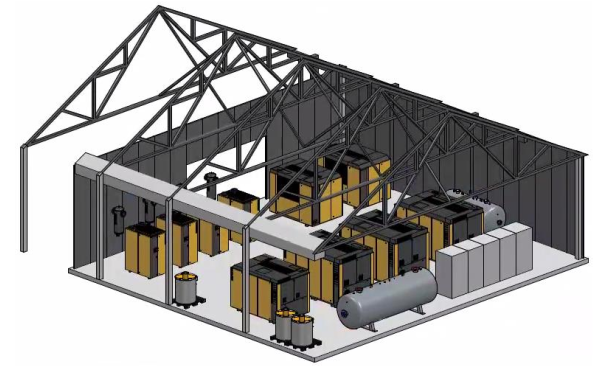
\includegraphics[width=\columnwidth]{cmpc_layout.png} \\
{\small \textcolor{DarkGray}{Layout de la sala de compresores (Anexo C del informe), base para el diseño del piping y la integración de equipos.}\par}


\end{multicols}

\end{sloppy} % <-- CAMBIO: Final del entorno sloppy.

% --- PIE DE PÁGINA: CONTACTO Y LLAMADA A LA ACCIÓN ---
\vspace*{\fill} % Empuja el pie de página hasta el fondo
\color{OrangeAccent}\rule{\linewidth}{1.5pt}
\vspace{2mm}
\begin{center}
\textcolor{DeepBlue}{\large\textbf{¿Enfrenta un desafío de ingeniería similar? Conversemos.}} \
\vspace{1mm}
\textcolor{DarkGray}{
\faLinkedin\ \href{https://www.linkedin.com/in/felipewasaff/}{in/felipewasaff} \quad
\faEnvelope\ \href{mailto:felipe.wasaff@wasaffconsulting.com}{felipe.wasaff@wasaffconsulting.com} \quad
\faGlobe\ \href{https://www.wasaffconsulting.com}{wasaffconsulting.com}
}
\end{center}
\end{document}